\documentclass[10pt]{beamer}
\usepackage{kotex}

\usepackage{framed}
\usepackage{graphicx}
%https://www.overleaf.com/learn/latex/Inserting_Images

\usepackage{amsmath}
%use dfrac
\usepackage{xcolor}

\usepackage{amsthm}
%\usepackage{tabl}
\usepackage{listings}
\definecolor{mGreen}{rgb}{0,0.6,0}
\definecolor{mGray}{rgb}{0.5,0.5,0.5}
\definecolor{mPurple}{rgb}{0.58,0,0.82}
\definecolor{backgroundColour}{rgb}{0.95,0.95,0.92}
%https://tex.stackexchange.com/questions/348651/c-code-to-add-in-the-document
\lstdefinestyle{CStyle}{
    backgroundcolor=\color{backgroundColour},   
    commentstyle=\color{mGreen},
    keywordstyle=\color{magenta},
    numberstyle=\tiny\color{mGray},
    stringstyle=\color{mPurple},
    basicstyle=\footnotesize,
    breakatwhitespace=false,         
    breaklines=true,                 
    captionpos=b,                    
    keepspaces=true,                 
    numbers=left,                    
    numbersep=5pt,                  
    showspaces=false,                
    showstringspaces=false,
    showtabs=false,                  
    tabsize=2,
    language=C
}


\usepackage{etoolbox}
\AtBeginEnvironment{quote}{\singlespacing\small}


\usepackage{thmtools}
\usepackage{xcolor}
\declaretheoremstyle[% spaceabove=6pt,spacebelow=6pt, headfont=\color{MainColorOne}\sffamily\bfseries, notefont=\mdseries, notebraces={[}{]}, bodyfont=\normalfont,
headpunct={},
postheadspace=1em,
%qed=▣,
]{maintheorem}

\declaretheorem[%
name=정의,
style=maintheorem,
numberwithin=section, shaded={%bgcolor=MainColorThree!20,
margin=.5em}]{dfn}
% \begin{dfn}[]
% \end{dfn}


\usetheme{Hannover}


\title{String Matching}

\author{EUnS}

\begin{document}

\begin{frame}
  \maketitle
\end{frame}


\begin{frame}{Preface}
    \begin{figure}[h!]
        \centering
        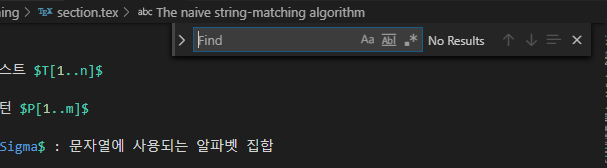
\includegraphics[scale=0.6]{pre1.PNG}
        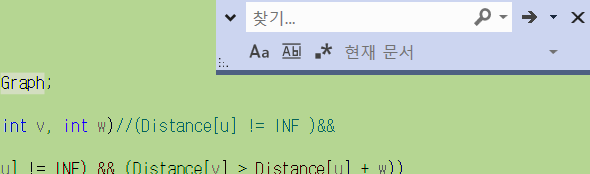
\includegraphics[scale=0.6]{pre2.PNG}
    \end{figure}
\end{frame}



\section{The naive string-matching algorithm}



\begin{frame}[fragile]{주먹구구}
    각 $k$마다 $T[k]$부터 $T[k+m-1]$까지 하나하나 $P$와 맞는지 확인하는것이다.
\begin{lstlisting}[style = CStyle]
NAIVE-STRING-MATCHER (T,P)
    n = T.length
    m = P.length
    for s = 0 to n-m
        if(P[1..m] == T[s+1..s+m])
            print ``Pattern occurs with shift s"
\end{lstlisting}
\end{frame}

\begin{frame}
    매칭시간 $O((n-m+1)m)$ 좀 더 줄일수 없나?
\end{frame}



\begin{frame}
    \tableofcontents
\end{frame}


\begin{frame}
    \frametitle{약속}
    \begin{itemize}
        \item 텍스트 $T[1..n]$ 
        \item 패턴 $P[1..m]$
        \item $\Sigma$ : 문자 집합 (영어, 한국어, 중국어..)
    \end{itemize}
\end{frame}



\section{The Rabin-Karp algorithm}

\begin{frame}
    \frametitle{idea}
    문자를 숫자로 바꾸자!
\end{frame}


\begin{frame}
    \begin{figure}[h!]
        \centering
        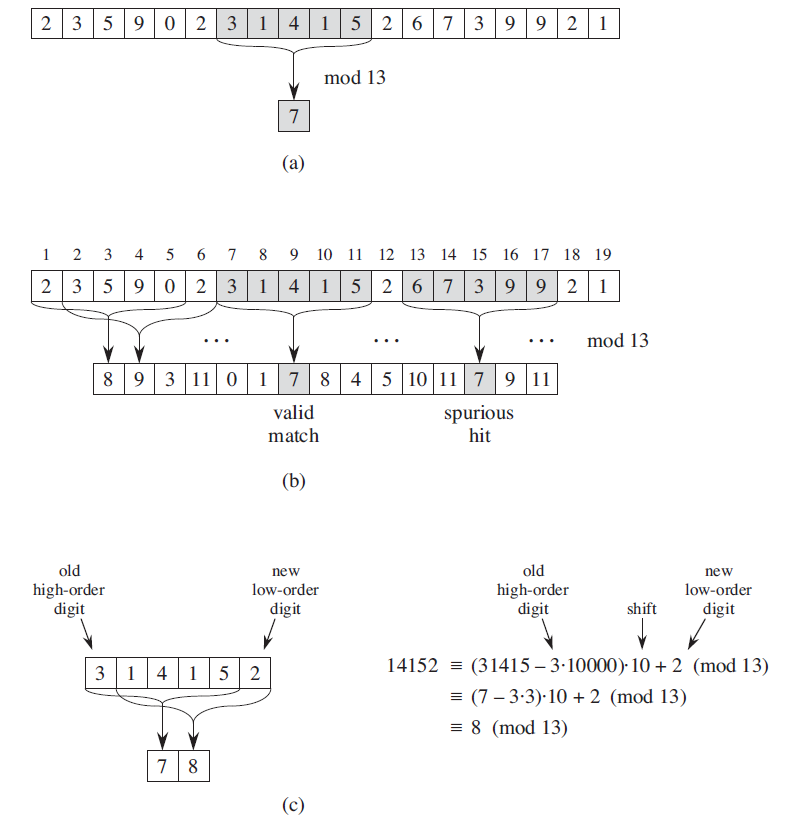
\includegraphics[scale=0.4]{pic1.PNG}
    \end{figure}
\end{frame}



% \begin{frame}

%     $q$를 채용한다.그래서 그 나타낸 숫자가 매칭이 이루어졌을때 실제로 같은 문자열인지 검사하는 부분이 필요하다. 
%     이 $q$는 일반적으로 $dq$가 컴퓨터 한워드에 들어가는 소수로 채용한다.

% \end{frame}


\begin{frame}
    \frametitle{호너의 법칙(Horner's law)}
    
    $\Theta(m)$
    
    $$p = P[n]+ d(P[n-1] + d(P[n-2]+ \cdots + d(P[2] + d(P[1])) \cdots )) \bmod q $$

    $$p = (dp+P[i]) \bmod q$$
    
    문자열 $T[s+1..s+m]$에 대한 숫자 $t_s$의 처리는 매칭과 직후에 계산 한다.
    
    $$t_{s+1} = (d(t_s - T[s+1]h) + T[s+m+1]) \bmod q$$
\end{frame}





\begin{frame}[fragile]

\begin{lstlisting}[style = CStyle]
RABIN-KARP-MATCHER(T,P,d,q)
    n = T.length
    m = P.length
    h = d^{m-1} mod q
    p = 0
    t_0 = 0
    for( i = 1 to m)
        p = (dp+P[i])mod q
        t_0 = (dt_0 + T[i]) mod q
    for s = 0 to n-m
        if p == t_s
            if P[1..m] == T[s+1..s+m]
                print ``Pattern occurs with shift s"
        if s < n - m
            t_{s+1} = (d(t_s - T[s+1]h) + T[s+m+1]) mod q
\end{lstlisting}
    


\end{frame}

\begin{frame}
    \begin{itemize}
        \item 전처리 $\Theta(m)$
        \item 매칭시간 $O((n-m+1)m)$
    \end{itemize}
    
    아쉬운 점 : 여전히 완벽하게 일치하는지 확인하기 위해 하나하나 비교하는 방법을 사용한다.
\end{frame}




\section{String matching with finite automata}

\begin{frame}
\begin{dfn}[automata]
    finite automaton은 다음과 같이 5개의 튜플로 구성된다.
    \begin{itemize}
        \item $Q$ : 유한 상태의 집합
        \item $q_0$ :시작 상태 ($q_0 \in Q$)
        \item $A$ : 받아들이는 상태의 구분된 상태 ($A \subset Q$)
        \item $\Sigma$ : 유한 입력 알파벳 집합
        \item $\delta$ : $Q \times \Sigma$에서 $Q$로 매핑되는 전이 함수 $M$    \end{itemize}
\end{dfn}
\end{frame}



\begin{frame}
        
    뭔소린지모르겠죠?

    저도 그럼

    오토마타 내용 통째로 생략

\end{frame}


\begin{frame}
    \frametitle{$\delta$ 상태표란}
    \begin{itemize}
        \item 문자열 $T$는 각 자리마다 상태를 가진다.
        \item 초기 시작 상태는 0
        \item 현재 문자의 상태는 문자의 상태와 현재 문자에 따라 정해진다.
        \item 상태는 상태표를 보고 정한다.
    \end{itemize}
\end{frame}


\begin{frame}
    \frametitle{$\delta$ 상태표를 구해라}
    \begin{enumerate}
        \item 상태 : 앞에서부터 각각의 문자가 가장 길게 일치하는 갯수
        \item $(m+1) \times \Sigma$ 배열
        \item 상태가 $m$에 도달하면 매칭
    \end{enumerate}
\end{frame}


\begin{frame}
    \begin{figure}[h!]
        \centering
        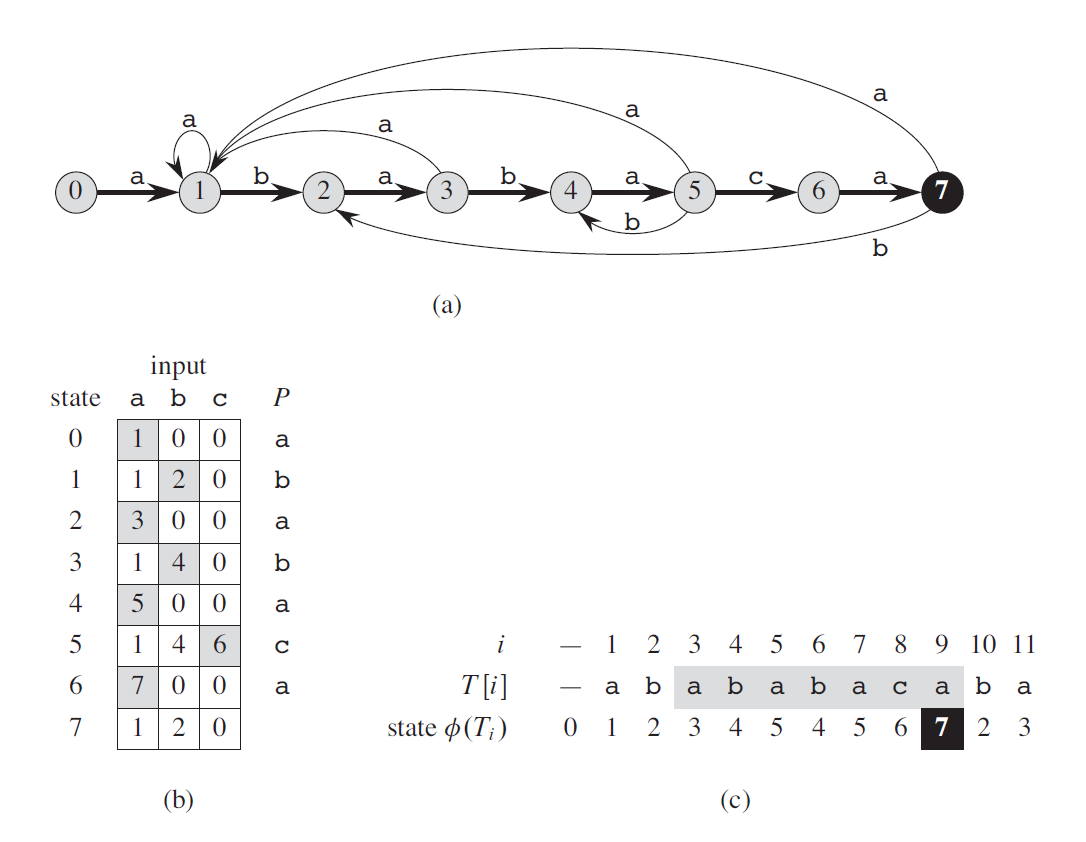
\includegraphics[scale=0.4]{pic2.PNG}
        \caption{$|\Sigma|  = 3$ ``a,b,c", $m = 7$}
    \end{figure}
\end{frame}




\begin{frame}[fragile]
\begin{lstlisting}[style = CStyle]
FINITE-AUTOMATON-MATCHER(T, delta , m)
n = T.length
q = 0 
for i = 1 to n
    q = d(q,T[i])
    if q == m
        print ``Pattern occurs with shift i-m"
\end{lstlisting}
\end{frame}




\begin{frame}[fragile]
\begin{lstlisting}[style = CStyle]
COMPUTE-TRANSITION-FUNCTION(P, Sigma)
    m = P.length
    for q = 0 to m
        for a in Sigma
            k = min(m+1,q+2)
            repeat 
                k = k - 1
                until P_k ] P_q-a
                d(q,a) = k
    return d
\end{lstlisting}
\end{frame}


% 상태표를 구하기위해서 다음과 같이 진행한다.
% 각 상태 $q$ 마다 각 알파벳 $a$를 뽑는다.
% 현재 상태 $q$의 문자열 + 'a'가 임의의 상태 $k$를 끝에서 포함하는지 검사하고 다를시 $k$를 계속 낮춰간다.


\begin{frame}
    \begin{itemize}
        \item 전처리의 수행시간 $O(m^3 \Sigma)$
        \item 상태표의 공간 복잡도의 크기가 $\Theta(m|\Sigma|)$
        \item $\Theta(n)$
    \end{itemize}
\end{frame}

\begin{frame}
    \begin{itemize}
        \item 뒷절의 $KMP$방식을 차용해서 전처리 시간을 $O(m \Sigma)$로 개선할수있다.
        \item 공간 복잡도의 크기를 더 줄여보자.    
    \end{itemize}
\end{frame}








\section{The KMP algorithm}

\begin{frame}{KMP?}
    \begin{itemize}
        \item Knuth-Morris-Pratt이 공동 발표한 알고리즘
    \end{itemize}
\end{frame}


\begin{frame}{샛길}
    \framesubtitle{Donald Knuth}
    \begin{figure}[h!]
        \centering
        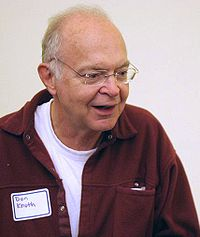
\includegraphics[scale=0.7]{pic5}
        %\caption{}
    \end{figure}
    \begin{itemize}
        \item TAOCP(The art of computer programing)의 저자 
        
        1968에 첫권이나오고 총 7권 계획인데 이제 책이 4권 출시됨 
        각종 알고리즘 논문 참고로 빠짐없이 개근상.
        \item TEX 창시자
        \item 각종 CS 책에 심심하면 거론되는 인물
    \end{itemize}
\end{frame}



\begin{frame}
    \frametitle{$\delta$대신 $\pi$}
    \begin{itemize}
        \item 크기 $m$
        \item 매칭이 실패했을때 사용.
        \item 앞의 문자열과 가장 근접하게 일치하는 위치를 반환
    \end{itemize}
\end{frame}



\begin{frame}
    \begin{figure}[h!]
        \centering
        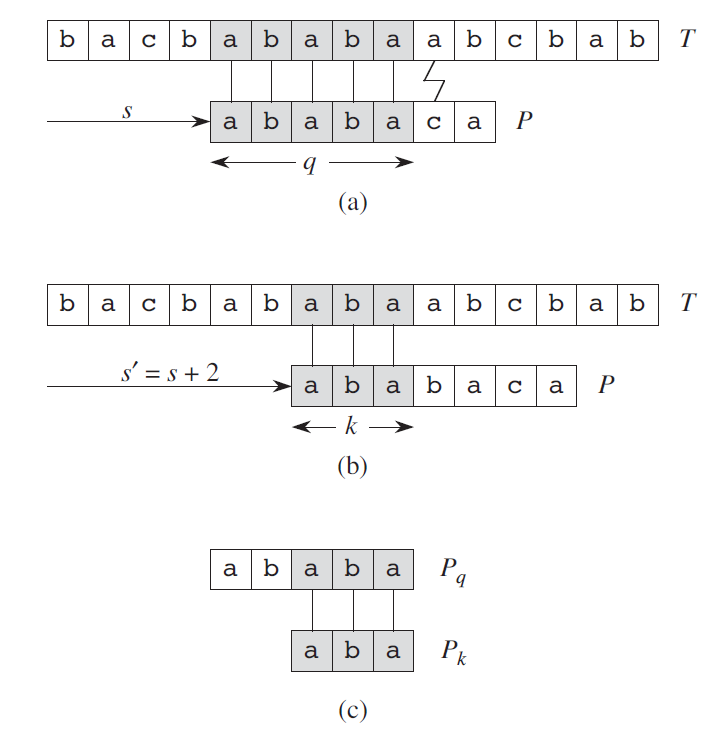
\includegraphics[scale=0.4]{pic3.PNG}
        %\caption{}
    \end{figure}
\end{frame}



\begin{frame}
    \begin{figure}[h!]
        \centering
        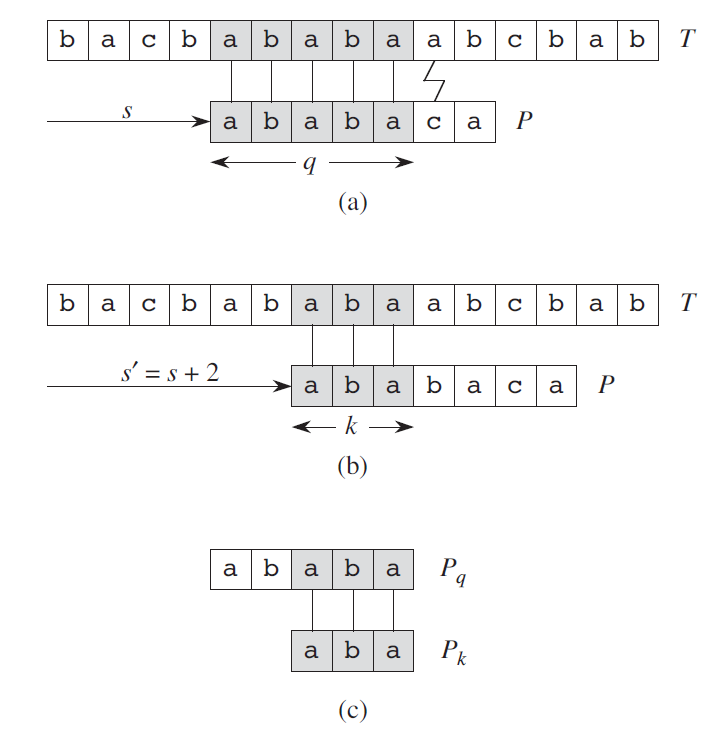
\includegraphics[scale=0.4]{pic3.PNG}
        %\caption{}
    \end{figure}

\end{frame}


\begin{frame}
    \begin{figure}[h!]
        \centering
        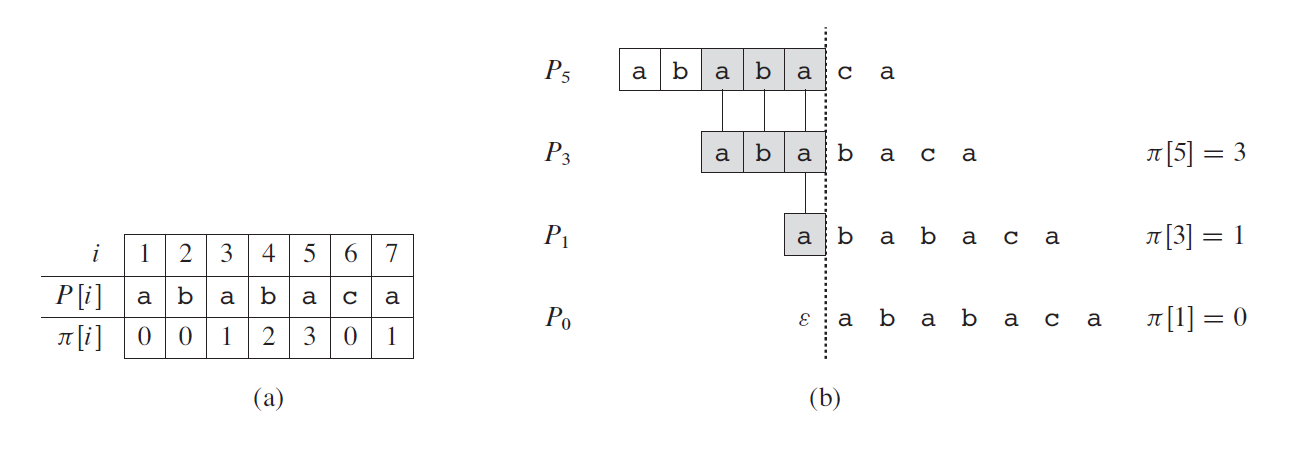
\includegraphics[scale=0.3]{pic4.PNG}
        \caption{(a)는 패턴 $P$와 전처리한 $\pi[1..7]$ (b)는 $P[5]$에서 다음 문자가 매칭이 틀렸을때 그에 따른 $\pi$값과 되돌아가는 순서를 나타낸것이다.}
    \end{figure}
\end{frame}

\begin{frame}[fragile]
\begin{lstlisting}[style = CStyle]
KMP-MATCHER(T,P)
    n = T.length
    m = P:length
    PI[] = COMPUTE-PREFIX-FUNCTION(P)
    q = 0 // number of characters matched
    for i = 1 to n // scan the text from left to right
        while q>0 and P [q+1] != T[i]
            q = PI[q] // next character does not match  
        if P [q+1] == T[i]
            q = q + 1 // next character matches
        if q == m // is all of P matched?
            print ``Pattern occurs with shift" i - m
            q  = PI[q]
\end{lstlisting}
\end{frame}




\begin{frame}[fragile]
\begin{lstlisting}[style = CStyle]
COMPUTE-PREFIX-FUNCTION(P) /
    m = P.length
    let PI[1..m] be a new array
    PI[1] = 0
    k = 0
    for q = 2 to m
        while k>0 and P[k+1] != P[q]
            k = P[k]
        if P[k+1] == P[q]
                k = k + 1
        PI[q] = k 
    retunr PI
\end{lstlisting}

\end{frame}



\begin{frame}
    \begin{itemize}
        \item 전처리 : $O(m)$
        \item 매칭시간 : $\Theta(n)$
    \end{itemize}
\end{frame}

%http://yoonkn.blogspot.com/2009/06/beamer-에서-table-쓰기-한프레임안에-큰테이블-구겨넣기.html

\section{conclusion}

\begin{frame}
    \frametitle{정리}
    \begin{center}
        \begin{tabular}{| c | c | c | c |}
          \hline \hline
          알고리즘 & 전처리 & 수행시간     & 공간복잡도               \\   \hline
          naive & 0 &   $O((n-m+1)m)$   & 0         \\ \hline
          Rabin-Karp &$\Theta(m)$     & $O((n-m+1)m)$   &    $\Theta(1|)$      \\   \hline
           finite automata & $\Theta(m \Sigma)$  &  $\Theta(n)$ & $\Theta(m|\Sigma|)$ \\ \hline
          The KMP algorithm & $\Theta(m)$ &  $\Theta(n)$   &  $\Theta(m)$   \\   
          \hline\hline
        \end{tabular}
    \end{center}

    % \item 전처리의 수행시간 $O(m^3 \Sigma)$
    % \item 상태표의 공간 복잡도의 크기가 $\Theta(m|\Sigma|)$
    % \item $\Theta(n)$
    % 전처리 : $O(m)$  매칭시간 : $\Theta(n)$
\end{frame}


\begin{frame}
    \begin{center}
     \textrm{   There's no such thing as a stupid question.    }
    \end{center}
\end{frame}


\end{document}
